\begin{IEEEbiography}[{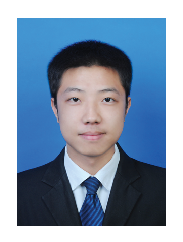
\includegraphics[width=1in,height=1.25in,clip,keepaspectratio]{author1-zhongkai.eps}}]
{Kai Zhong}
received the PhD degree in computer science from Hunan University, Changsha, China, in 2024. He is currently a postdoctoral researcher at Hunan University. His research interests include cybersecurity, industrial control systems, and edge-cloud computing.
\end{IEEEbiography}
\vspace{-2mm}
\begin{IEEEbiography}[{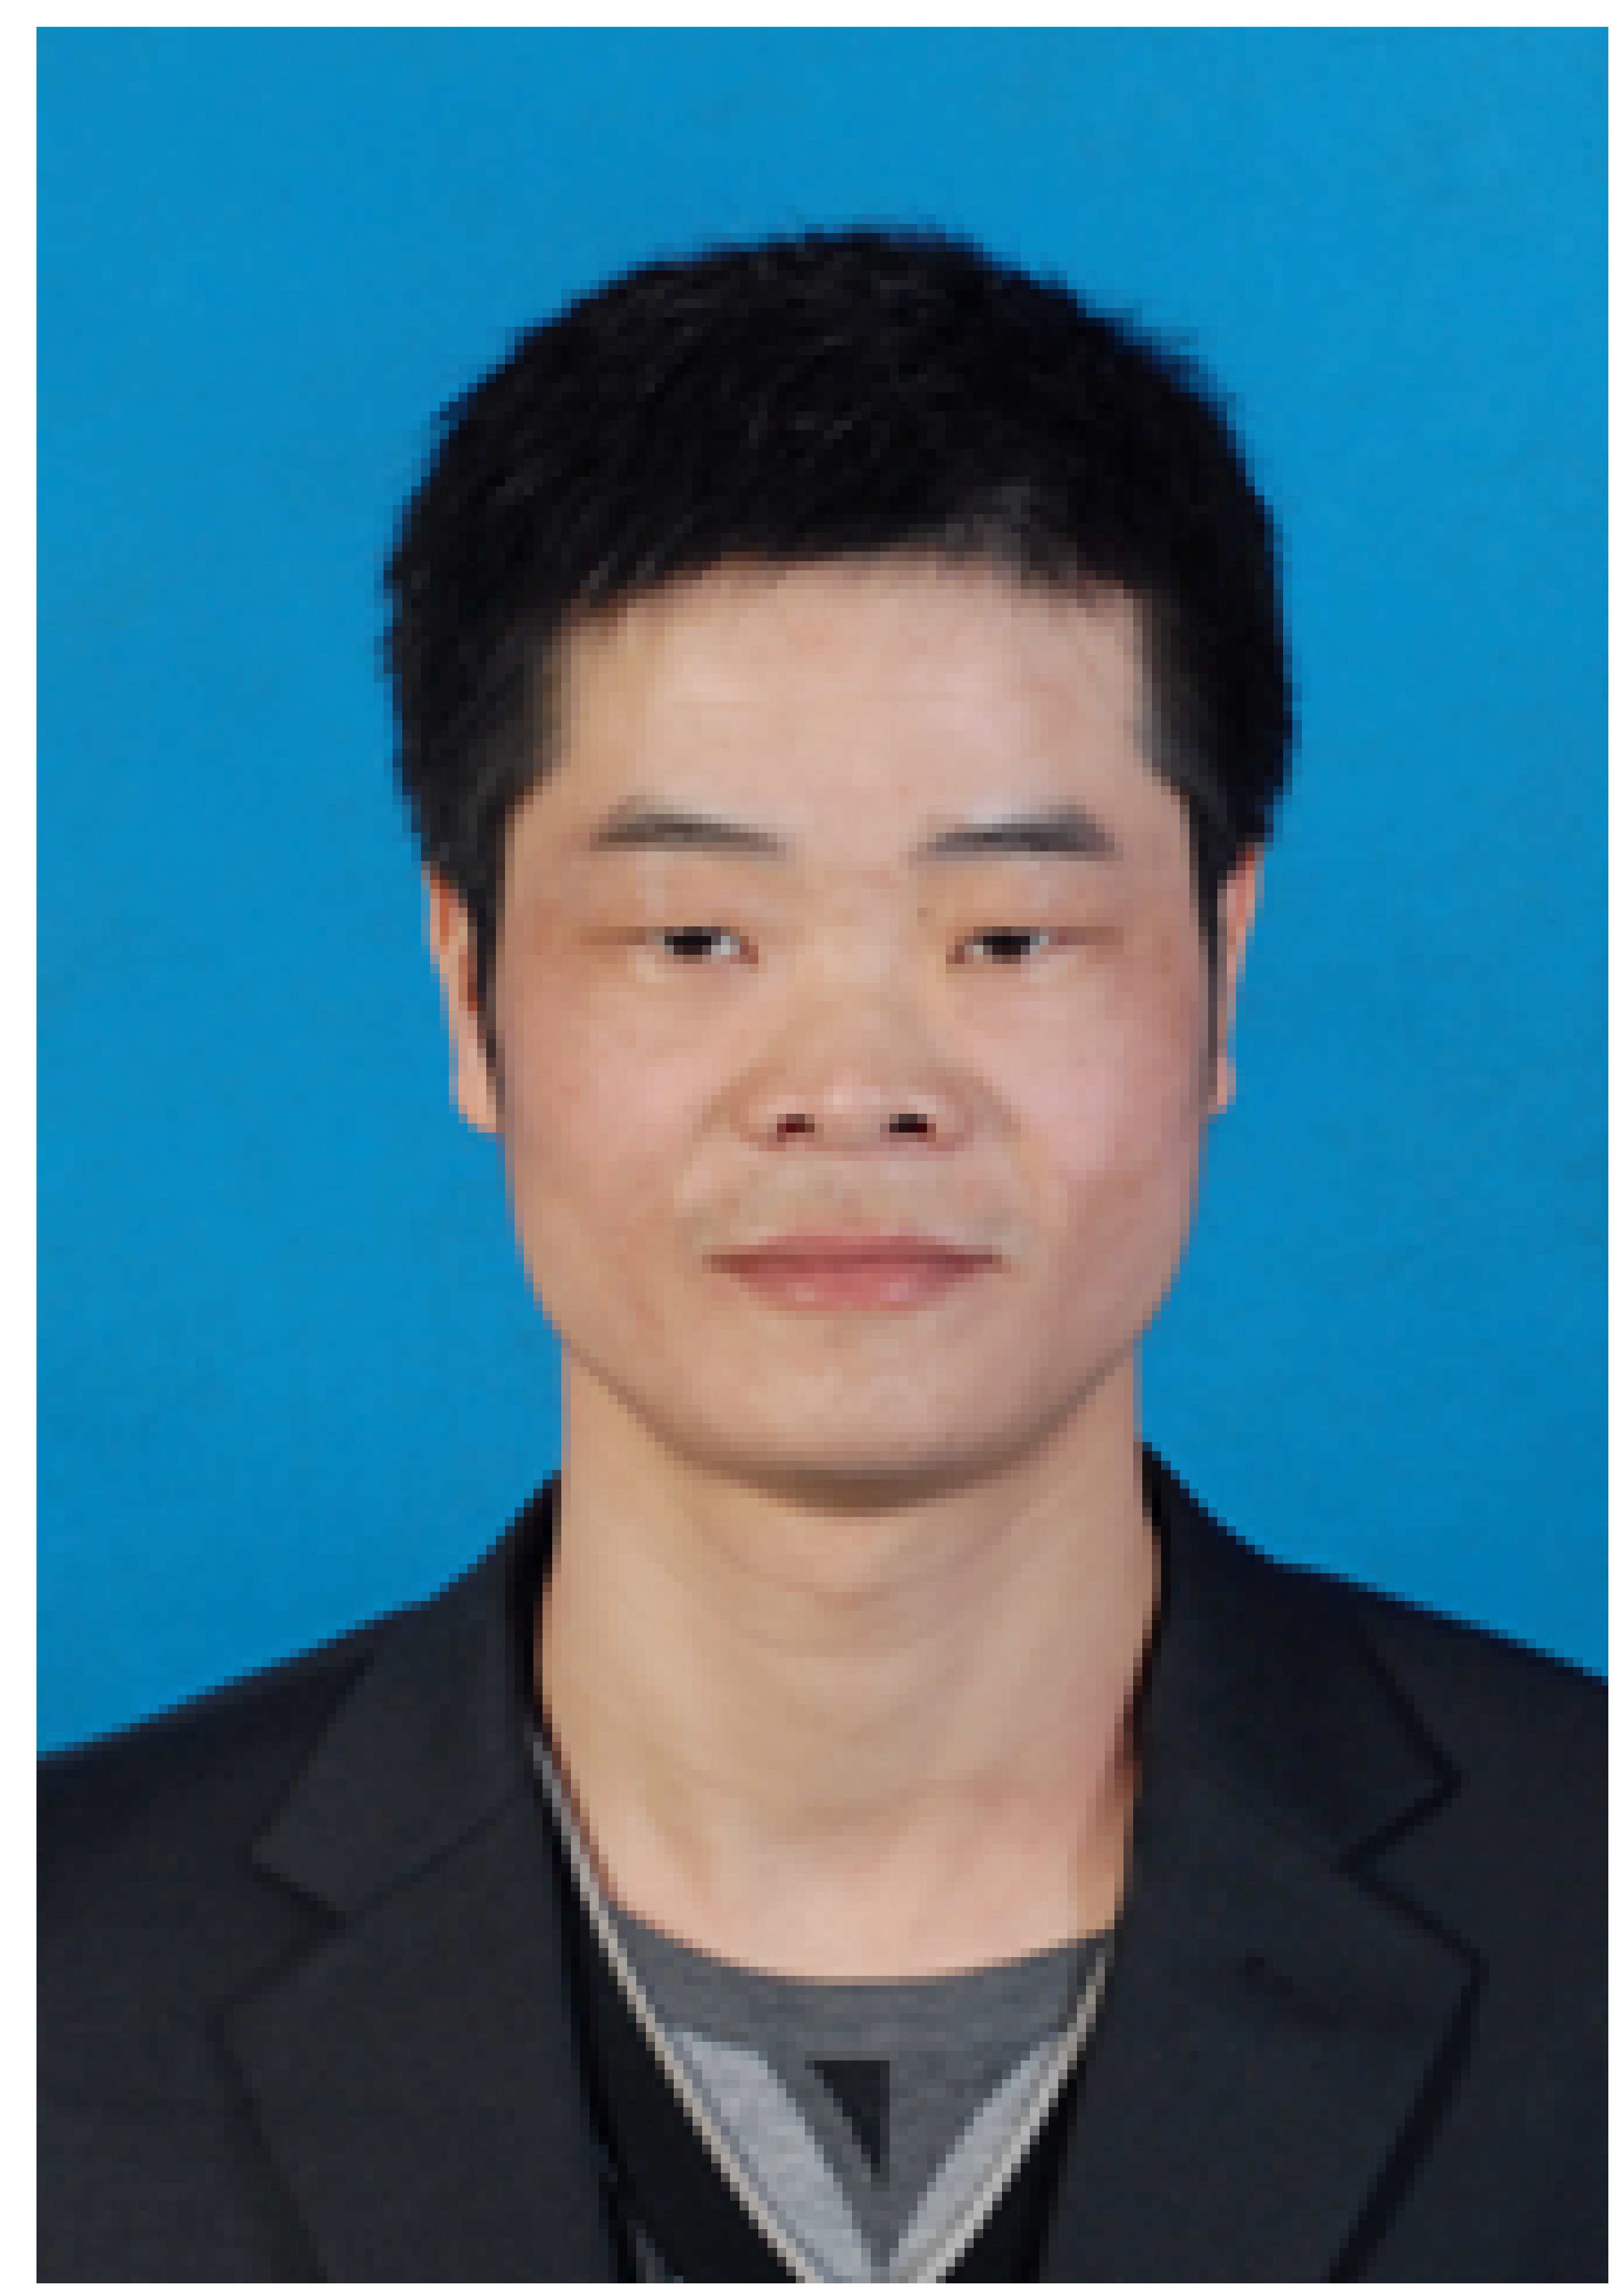
\includegraphics[width=1in,height=1.25in,clip,keepaspectratio]{author2-yangzb.eps}}]
{Zhibang Yang}
received the PhD degree in computer science from Hunan University, Changsha, China, in 2012. He is currently an associate professor at Changsha University. His research interests include cybersecurity, industrial control systems, and edge-cloud computing.
\end{IEEEbiography}
\vspace{-2mm}
\begin{IEEEbiography}[{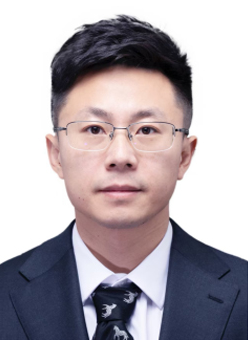
\includegraphics[width=1in,height=1.25in,clip,keepaspectratio]{yumeng.png}}]{Yumeng~Liu} 
received the PhD degree from the Institute of Software, Chinese Academy of Sciences, Beijing, China, in 2023. He is a senior engineer at the Institute of Software, Chinese Academy of Sciences. His research interests include data mining and database technology.
\end{IEEEbiography}
\vspace{-2mm}
\begin{IEEEbiography}[{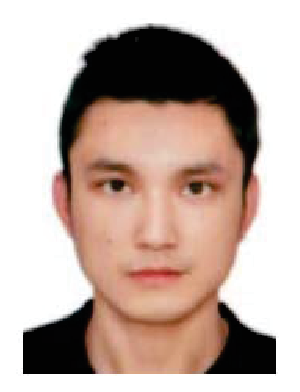
\includegraphics[width=1in,height=1.25in,clip,keepaspectratio]{author3-yusiyang.eps}}]{Siyang Yu} 
	received the PhD degree in computer science and technology from Hunan University, China, in 2017. He is currently a faculty member at Hunan University of Finance and Economics. His research interests include the industrial Internet of Things, anomaly analysis, and intrusion detection.
\end{IEEEbiography}
\vspace{-2mm}
\begin{IEEEbiography}[{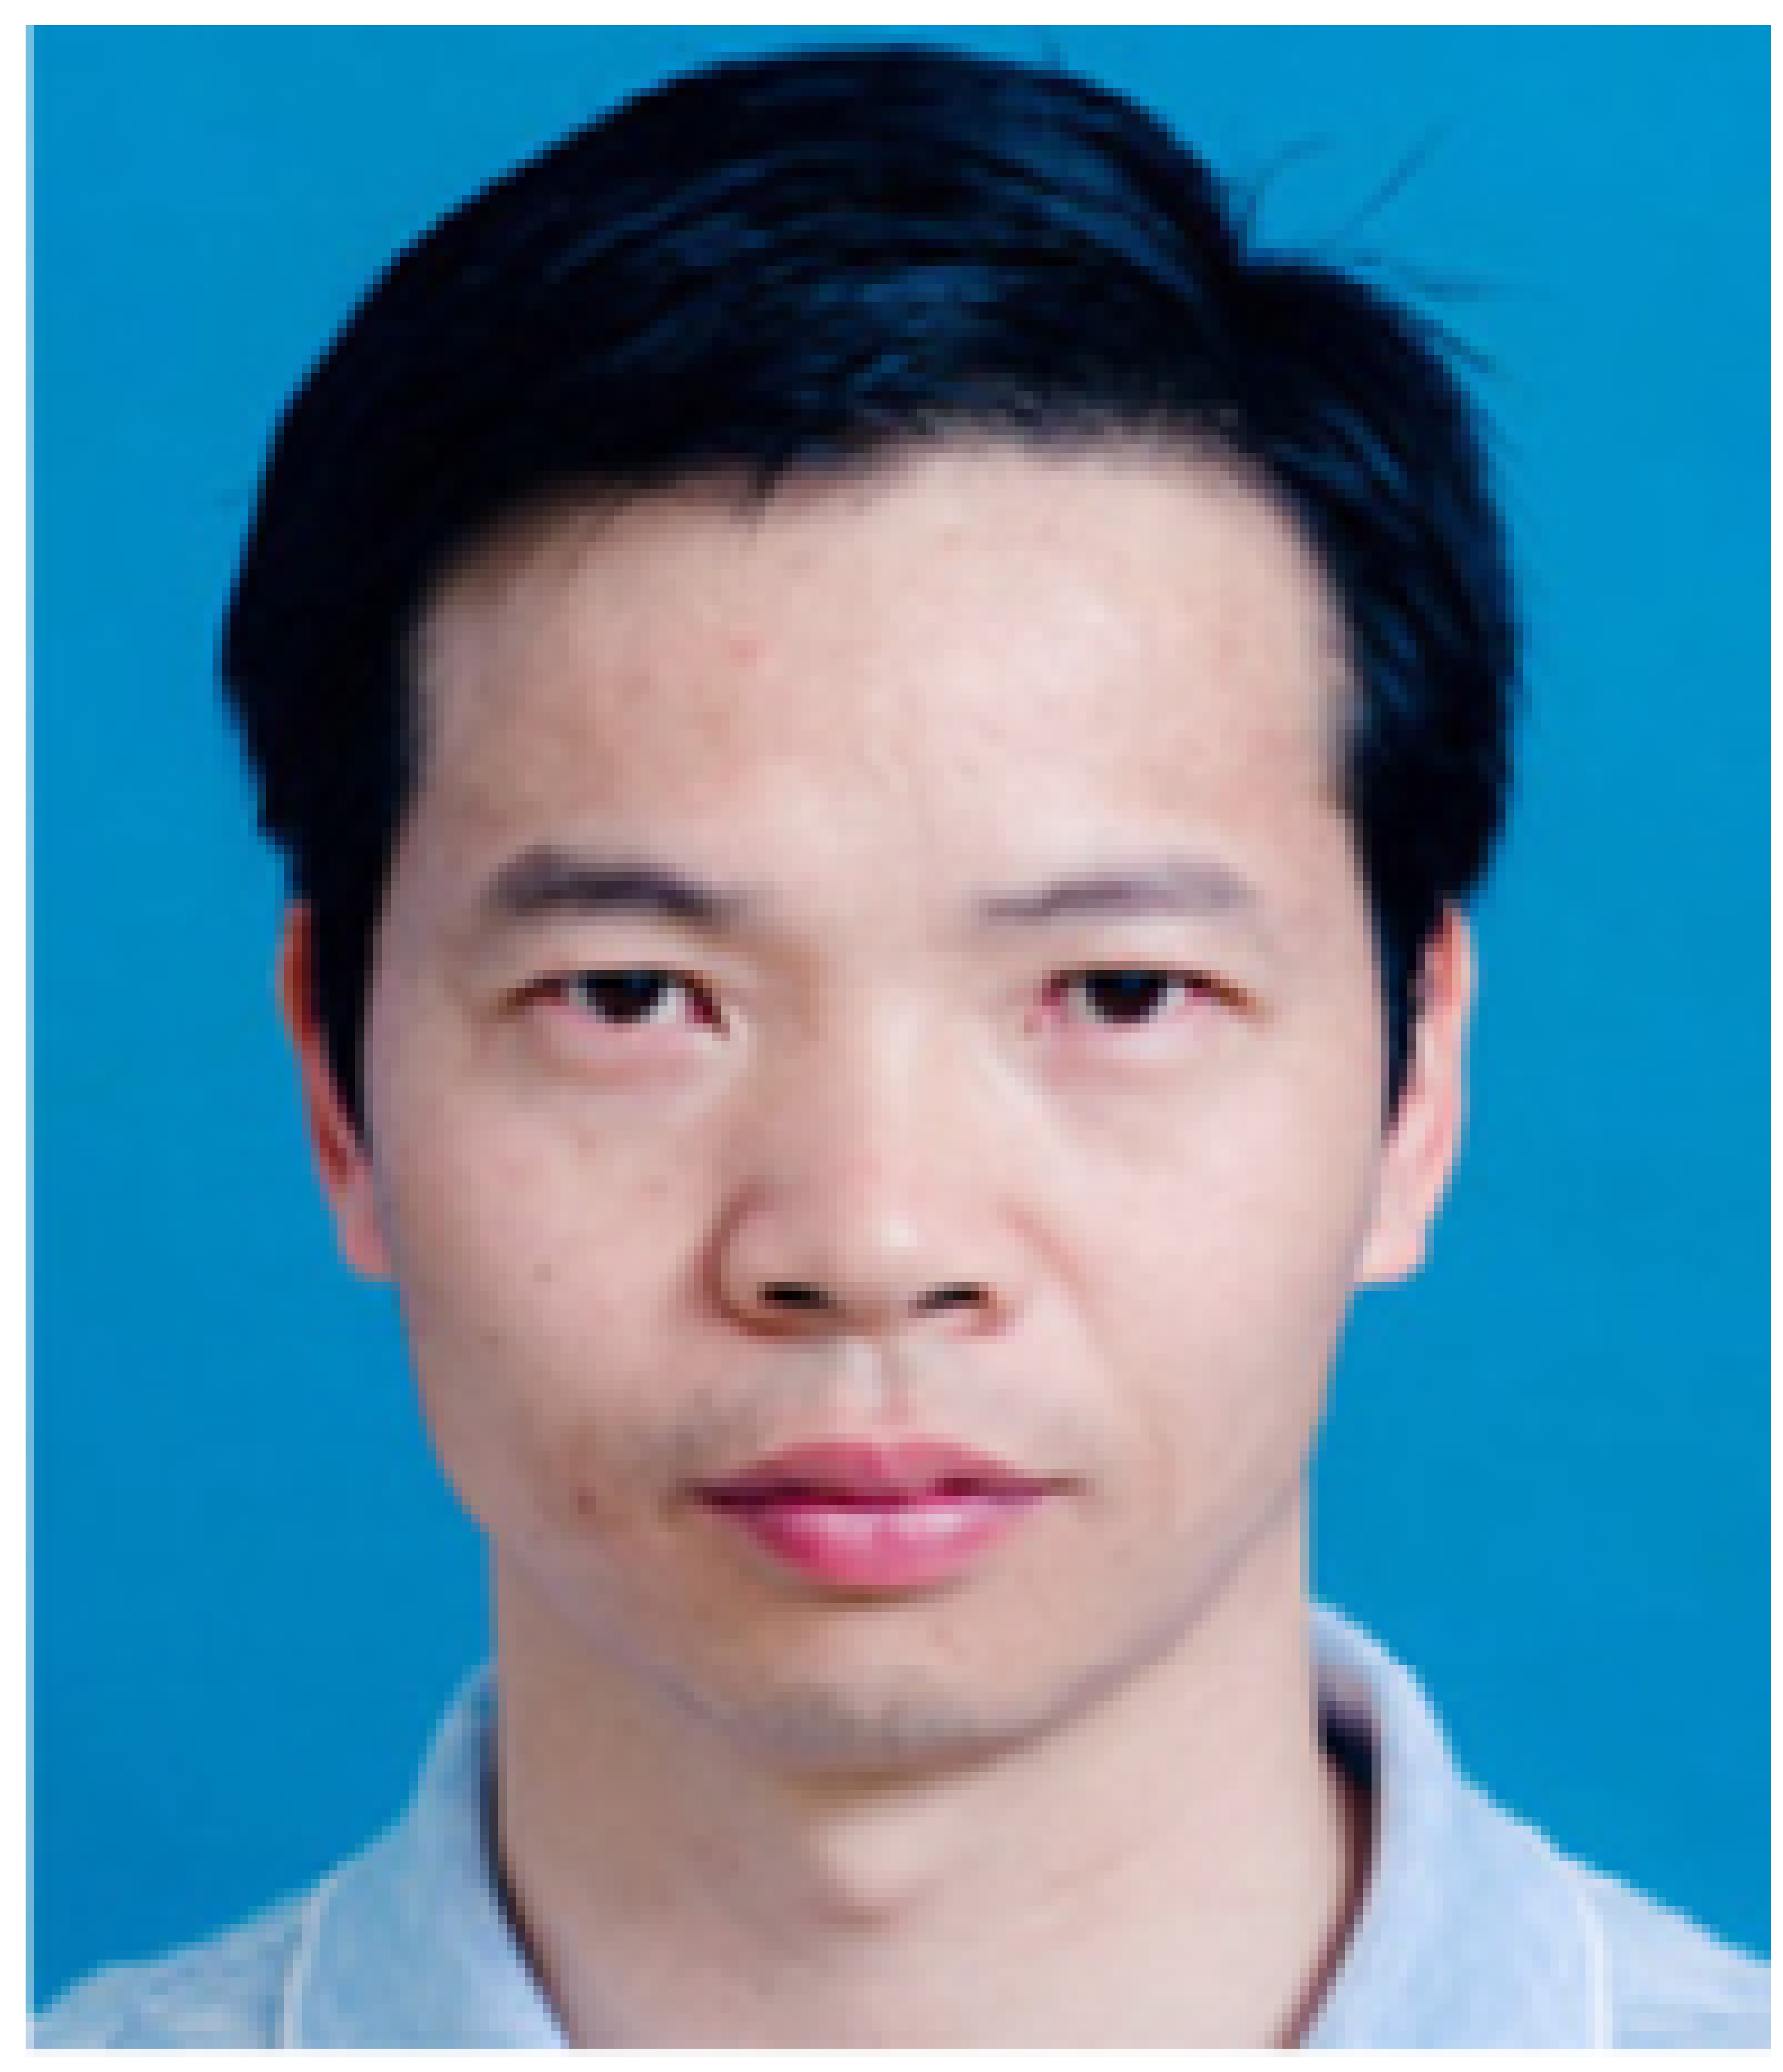
\includegraphics[width=1in,height=1.25in,clip,keepaspectratio]{author4-liKenli.eps}}]{Kenli Li}
	received the PhD degree in computer
	science from Huazhong University of Science
	and Technology, China, in 2003. He is currently a Cheung Kong professor of computer science and technology with Hunan University and the dean of the College of Computer Science and Electronic Engineering, Hunan University. His research interests include parallel and distributed processing, high-performance computing, and big data management. He has published more than 250 research papers
	in international conferences and journals such as TC, TPDS, TCC, ICPP, ICDCS, etc.
	He serves on the editorial board of the IEEE-TC. He is an outstanding member of the CCF and a senior member of the IEEE.
\end{IEEEbiography}




